\clearpage

\setlength{\headsep}{10mm}

\pagestyle{fancy}
\fancyhf{}
\renewcommand{\headrulewidth}{0pt}
\cfoot{\thepage}
\chead{\textsc{\nouppercase{\leftmark}}}

\section{Introduction}\label{ch:intro}

With primary motivations covered in the \hyperlink{prologue}{Prologue}, this introduction provides an overview of this thesis by chapter and section, highlighting more specific motivations behind these and main results within them. When it is clear to do so, background mathematics and related literature is also provided in this overview, rather than in the following core chapters' context.

The only background needed at the moment is notational: following convention, $\uC$ and $\uD$ will be used to denote sets of continuous and c\`adl\`ag functions, e.g.~like in \cite{billingsley_1999}. Extending this, $\uC_0^1$ denotes first-order differentiability and that all functions start from zero.

\vspace{3mm}\textbf{From the Heston model to ODEs.} This thesis is generally presented from foundations to applications. With the preliminary Heston-related goals discussed in the \hyperlink{prologue}{Prologue} constituting one of the final applications, specifically covered in \autoref{sec:price_limits}, the connection of both \autoref{chap:wellposed} and \autoref{chap:solutions} with conventional volatility modelling, let alone the specific Heston model, may not be clear without this introductory explanation. Indeed, given that the volatility of a price is conventionally a probabilistic and model-dependent object, it is not until \autoref{sec:base_frame} that this process is defined within our framework, and not until \autoref{sec:heston_frame} that the earlier probability-free ODE analysis is precisely related to the Heston model.

We now forgo some precision in order to help develop readers' intuition for how classical stochastic volatility models like Heston's can be related on a pathwise basis to the ODEs treated in this thesis, and therefore how these ODEs can be related to volatility. Towards this, fix a probability space $(\Omega,\cF,\PP)$ which supports a standard 2d Brownian motion $W=(W^0,W^1)$ over $\RR_+$, and let $S=\{S_t\}_{t\in\RR_+}$ be the Heston price process constructed from $W$ and parameters $\sigma,\kappa,\theta,v>0$, $\rho\in[-1,1]$ as in \autoref{eq:heston_prologue}, i.e.~verifying the It\^o SDEs
\begin{equation}\label{eq:heston_intro}
    \dd V_t = \sigma\sqrt{V_t}\dd W^1_t + \kappa(\theta - V_t)\dd t,\quad \dd S_t = \sqrt{V_t}S_t\dd W^{\rho}_t,\quad (V_0,S_0) := (v,1).
\end{equation}
We may explicitly write this CIR SDE for $V$ in its integrated form starting from time zero, and solve the SDE for $S$ in terms of $V$ to obtain the equivalent model representation
\begin{equation}\label{eq:heston_intro2}
    V_t = \sigma\int_0^t\sqrt{V_s}\dd W^1_s + \kappa\int_0^t(\theta - V_s)\dd s + v,\quad S_t = \exp\left(\int_0^t\sqrt{V_s}\dd W^{\rho}_s-\frac12\int_0^t V_s\dd s\right).
\end{equation}
Now using a result due to \cite{dambis_1965} and \cite{dubins_1965}, stated precisely in \autoref{thm:DDS} and applied in \autoref{thm:heston_ode}, we may again write this model equivalently as
\begin{equation}\label{eq:tce}
    V_t = \sigma B^1_{\int_0^t V_s\dd s} + \kappa\left(\theta t - \int_0^t V_s\dd s\right) + v,\quad S_t = \exp\left(B^\rho_{\int_0^t V_s\dd s} - \frac12\int_0^t V_s\dd s\right)
\end{equation}
where $B=(B^0,B^1)$ is another standard 2d Brownian motion over $\RR_+$ on $(\Omega,\cF,\PP)$, connected with $W$ according to \autoref{lem:heston_timechange}, and $B^\rho$ is defined like $W^\rho$ by $B^\rho:=\rho B^1+\sqrt{1-\rho^2}B^0$.

The rich history of the `change of time' method which results in the representation of the CIR process $V$ in \autoref{eq:tce} is presented in \cite{swishchuk_2016}, with the general theory covered concisely in \cite{barndorff-nielsen_2010}. Although \cite{ikeda_1989} makes some important contributions, this line of research originates from the work of Wolfgang Doeblin, in 1940. Before It\^o's calculus, e.g.~the integral of \cite{ito_1944} and SDEs of \cite{ito_1951}, Doeblin had shown that diffusions like $V$ admit `time-changed' representations like that in \autoref{eq:tce}, even establishing properties of martingales before the concept existed. This is not widely known because Doeblin unfortunately died in 1940, and his work only discovered in 2000. See \cite{bru_2002} for the surprising history of Doeblin's work.

Specifically, in \autoref{eq:tce} we would call the integrated (or cumulative) variance process $\int_0^t V_s\dd s$ a `time-change' of $B^1$. Technically, a time-change must possess certain adaptedness properties related to stopping times, given precisely in \autoref{def:time_change}, but these, and related properties of martingales, are not important for the core analysis of this thesis, especially regarding the Heston and NIG relationship discussed in the \hyperlink{prologue}{Prologue}. So this is where, until \autoref{sec:martingale}, this thesis diverges from research related to changes of time and martingales, because we will more generally consider this process $\int_0^t V_s\dd s$ as a random ODE solution.

Towards this, there turns out to be nothing special about $B$ in \autoref{eq:tce}, so we can instead construct this model from the arbitrary Brownian motion $W$ on $(\Omega,\cF,\PP)$, and then define the process $X_t:=\int_0^t V_s\dd s$ to obtain another representation of a Heston price process
\begin{equation}\label{eq:tce2}
    X'_t = \sigma W^1_{X_t} + \kappa\left(\theta t - X_t\right) + v,\quad S_t = \exp\left(W^\rho_{X_t} - \tfrac12 X_t\right),
\end{equation}
where $X'_t:=\frac{\dd}{\dd t}X_t = V_t$. Now for each $(t,x)\in\RR^2_+$, define the real random variable $Y_{t,x}:= \sigma W^1_x + \kappa\left(\theta t - x\right) + v$, and the random field $Y=\{Y_{t,x}\}_{(t,x)\in\RR_+^2}$. A random field is just a random element of $\uC(\RR^2_+,\RR)$ which, drawing upon the text \cite{barndorff-nielsen_2018}, is defined precisely in \autoref{def:rand_field}. Now write \autoref{eq:tce2} succinctly as
\begin{equation}\label{eq:rand_ode}
    X'_t = Y_{t,X_t},\quad S_t = \exp\left(W^\rho_{X_t} - \tfrac12 X_t\right).
\end{equation}
The process $X$ thus verifies $X'_t=Y_{t,X_t}$ and $X_0=0$, and so we will define it to be a solution of the random IVP $x'=Y_{t,x}$, $x_0=0$, as in \autoref{def:rand_ivp}. It is through the study of such random IVPs that we have been able to strengthen and generalise the Heston and NIG relationship discussed in the \hyperlink{prologue}{Prologue}, and more generally develop a robust volatility modelling framework summarised by \autoref{eq:rand_ode}, but specified more precisely in \autoref{def:price_frame}.

Focusing now just on the process $X$, which we will always call a cumulative variance process even when not explicitly referring to a related price process $S$ like in \autoref{eq:rand_ode}, we may fix an outcome $\omega\in\Omega$ and, defining the fixed function $g:=Y(\omega)\in\uC(\RR^2_+,\RR)$, may analyse the deterministic IVP $x'=g(t,x)$, $x(0)=0$, and in particular look for a path $X(\omega):=\vp\in\uC^1_0(\RR_+,\RR)$ which verifies $\vp'(t)=g(t,\vp(t))$ over $\RR_+$. Then in the Heston case,
\begin{equation}\label{eq:hest_ode}
    g(t,x) := \sigma w(x) + \kappa\left(\theta t - x\right) + v,
\end{equation}
where $w:=W^1(\omega)\in\uC_0(\RR_+,\RR)$. At this point, if we were to remove the spatial influence of $w$ on $g$, by replacing $w(x)$ in \autoref{eq:hest_ode} by $w(t)$, then \emph{existing} ODE theory can establish a unique global solution $\vp$, since $g$ becomes spatially Lipschitz. In the reduced case where the reversion level $\theta$ coincides with the starting variance $v$, this unique solution is given by
\begin{equation}
    \vp(t) = v t + \sigma\int_0^te^{-\kappa(t-s)}w(s)\dd s.
\end{equation}
Whether $\theta=v$ or not, this solution can be interpreted as an integrated Ornstein-Uhlenbeck (OU) path, because after this replacement of $w(x)$ by $w(t)$, the counterpart of the CIR SDE in \autoref{eq:heston_intro} for $V$ is the simpler OU SDE which has $\sqrt{V_t}$ removed. It is unfortunate but not surprising that these simplifications, treated by existing theory, are not directly helpful for volatility modelling, because the OU `variance' paths $\vp'=V(\omega)$ can become negative.

New ODE theory is required if we want to understand whether the general Heston case in \autoref{eq:hest_ode} has a unique positive global solution and want to avoid placing impractically restrictive regularity constraints on the path $w\in\uC_0(\RR_+,\RR)$, such as Lipschitz continuity.

This makes a case for avoiding considerations of the Heston model on this pathwise ODE basis, and sticking to the It\^o SDEs in \autoref{eq:heston_intro}. However, we believe the benefits of this alternative endeavour now speak for themselves. A surprising consequence of our new ODE theory is that, in the Heston case of \autoref{eq:hest_ode}, the IVP $x'=g(t,x)$, $x(0)=0$ actually has a unique maximal solution $\vp$ \emph{for all} $w\in\uC_0(\RR_+,\RR)$. Loosely, a `maximal' solution is any which `reaches the boundary of $\RR_+\!\times\!\RR$', and one which also exists over $\RR_+$ is `global'.

This maximal solution turns out to \emph{always} be strictly increasing, so can always be used to meaningfully model a cumulative variance path $\vp$, with corresponding non-negative volatility $\sqrt{\vp'}$. Given that such functions $g$ need not have any spatial regularity properties, which is clear given the path $w$ in \autoref{eq:hest_ode} may be any in $\uC_0(\RR_+,\RR)$, we call these IVPs spatially irregular, and these can be used to model a counter-intuitively wide set of volatility paths.

In the case of \autoref{eq:hest_ode}, this maximal uniqueness not only extends to a global result if $w$ verifies the condition $\sup_{x\in\RR_+}\kappa x - \sigma w(x) = \infty$, more generally given by $\inf_{x\in\RR_+}g(t,x)<0$ for each $t\in\RR_+$, but the solution $\vp$, which defines a bijection in $\uC^1_0(\RR_+,\RR_+)$, is then bounded above by the strictly increasing c\`adl\`ag path $\bvp\in\uD(\RR_+,\RR_+)$ deriving from $g$ according to
\begin{equation}\label{eq:cadlag_bound_intro}
    \bvp(t) := \inf\{x>0:g(t,x)<0\}.
\end{equation}
Substituting the representation of $g$ from \autoref{eq:hest_ode}, this c\`adl\`ag path takes the form
\begin{equation}\label{eq:path_bound}
    \bvp(t) := \inf\{x>0: \kappa x - \sigma w(x) > \kappa\theta t + v\}.
\end{equation}
Now replacing the Brownian motion path $w := W^1(\omega)$ with the process $W^1$, and defining the c\`adl\`ag process $\bX$ on a pathwise basis by $\bX(\omega):=\bvp$, then from \autoref{eq:path_bound} we have
\begin{equation}\label{eq:ig_intro}
    \bX_t := \inf\{x>0: \kappa x - \sigma W^1_x > \kappa\theta t + v\}.
\end{equation}
Consulting \cite{applebaum_2009}, this process $\bX$ is non other than the IG L\'evy process, also with an IG-distributed random starting point $\bX_0>0$. So relatively succinctly, we have demonstrated how considering the Heston model on a pathwise basis using these spatially irregular ODEs could be helpful in determining how this model is related to the NIG L\'evy process. For clarity, as in \autoref{eq:nig_prologue}, the NIG process depends heavily on the IG process, just like the Heston price process depends on the integrated variance process $X_t:=\int_0^t V_s\dd s$.

The fact that the path $\bvp$ in \autoref{eq:path_bound} is a well-defined element of $\uD(\RR_+,\RR_+)$ for \emph{all} $w\in\uC_0(\RR_+,\RR)$ satisfying this condition of $\sup_{x\in\RR_+}\kappa x - \sigma w(x) = \infty$ provides some more intuition as to how this approach may generalise the Heston and NIG connection. Indeed, we will eventually understand how \emph{any} strictly increasing path in $\uD(\RR_+,\RR_+)$ can be constructed as a limit of our IVP solutions, so also any strictly increasing process $\bX$ with paths in $\uD(\RR_+,\RR_+)$ as a limit of \emph{random} IVP solutions, then any price process of type $S=\exp(W^\rho_\bX-\frac12 \bX)$.

\vspace{2mm}Now that the connection between the spatially irregular ODEs studied in this thesis and pathwise volatility modelling is clear, we move onto a detailed overview of the main results in each chapter and section, starting with the well-posedness foundations of such ODEs.

\vspace{3mm}\textbf{\autoref{chap:wellposed}: Well-posedness for spatially irregular ODEs.} The focus of this chapter is a class of first-order, one-dimensional ODEs $x'=f(t,x)$ where $f$ is a function in $\uC(\RR^2,\RR)$ with some additional simple properties. These properties are captured by the following set.
\begin{definition}[Set $\uF$ of functions]\label{def:driving_func}
    Let the subset $\uF\subset\uC(\RR^2,\RR)$ contain the functions $f$ such that $f(\cdot,x)$ is strictly increasing for every $x\in\RR$, and $f(\tau,\xi)>0$ for some $(\tau,\xi)\in\RR^2$.
\end{definition}

These properties given to the functions in $\uF$ constitute a balance between simplicity and generality when considering various possibilities which we know results in strictly increasing IVP solutions $\vp$. As discussed, this ensures $\vp$ can be used to model a price's cumulative variance path with a meaningful volatility $\sqrt{\vp'}$, given that $\vp'$ is then always non-negative. It is the fact that the functions in $\uF$ need not have any spatial regularity properties, e.g.~$f(t,\cdot)$ need not be Lipschitz or H\"older continuous, which, on the one hand puts these ODEs outside of classical theory, but on the other enables the modelling of a rich set of volatility paths.

Notice that the functions in $\uF\subset\uC(\RR^2,\RR)$ here differ from $g\in\uC(\RR_+^2,\RR)$ defined in \autoref{eq:hest_ode} and related to the Heston model. This is because, at this stage, we do not want to assume that solutions $\vp$ goes through $(0,0)\in\RR^2$, i.e.~verify $\vp(0)=0$, and are thereafter contained in $\RR^2_+$. Treating different initial values $(\tau,\xi)\in\RR^2$ turns out to be delicate, specifically when $f(\tau,\xi)=0$, so this chapter just focuses on IVPs related to $\uF$, with the next chapter simplifying this to IVPs related to functions $g$ in a subset $\uG\subset\uC(\RR_+^2,\RR)$ and with $(\tau,\xi)=(0,0)$, only once $\uF$ and arbitrary initial values $(\tau,\xi)\in\RR^2$ are fully understood.

As with the Heston model in \autoref{eq:heston_intro}, we will always be interested in solutions $\vp$ which go forwards in time from an initial, i.e.~present, state. This state is described by the values $\tau$, $\xi$ and $f(\tau,\xi)$, given the requirements $\vp(\tau)=\xi$ and $\vp'(\tau)=f(\tau,\xi)$ which $\vp$ must verify. Given these values, any `history' of a solution $\vp$ can be considered as being described by parameters like $\sigma,\kappa,\theta,v$ in \autoref{eq:hest_ode}, defining $f$. Only in \autoref{chap:solutions} will we briefly consider such histories over some interval $(T,\tau]$, which must solve a \emph{terminal} value problem (TVP) $x'=f(t,x)$, $x(\tau)=\xi$, to help understand the sensible values of $\tau$, $\xi$ and $f(\tau,\xi)$.

For a given IVP $x'=f(t,x)$, $x(\tau)=\xi$, it will prove vitally important to understand the \emph{maximum} domain $[\tau,T_*)$ over which a solution $\vp$ exists, i.e.~remains finite. This is because, when we move to a probabilistic setting where a stochastic process $X$ solves a random IVP as in \autoref{eq:tce2}, we must prohibit e.g.~having $X_t\xrightarrow{t\to T_*}\infty$ with positive probability for some $T_*<\infty$. This explosion would not only be unnatural, given the possible behaviour of a price process like $S_t=\exp(W^\rho_{X_t} - \frac12 X_t)$ as $t\to T_*$, but mathematically it is then not even clear how to give the sense in which these stochastic processes should actually be considered conventional stochastic processes, i.e.~to provide a function set and $\sigma$-algebra into which these objects define measurable maps from $(\Omega,\cF,\PP)$, so that probability can be conducted.

The problem of this chapter's focus is thus as follows, and given the importance of understanding maximum domains, \emph{maximal} solutions will always be emphasised. These differ from non-maximal solutions only through the final condition on $T_*\vee\sup_{t\in[\tau,T_*)}|\vp(t)|$ here.
\begin{problem}[IVPs of \autoref{chap:wellposed}]\label{prob:ivp}
    For $f\in \uF$ and $(\tau,\xi)\in\RR^2$ where $f(\tau,\xi)>0$, find a maximal solution $\vp\in\uC^1([\tau,T_*),\RR)$ of the IVP $x'=f(t,x)$, $x(\tau)=\xi$. By definition, this means $\vp$ verifies $\vp'(t)=f(t,\vp(t))$ for each $t\in[\tau,T_*)$, $\vp(\tau)=\xi$ and also $T_*\vee\sup_{t\in[\tau,T_*)}|\vp(t)|=\infty$.
\end{problem}

This maximal condition $T_*\vee\sup_{t\in[\tau,T_*)}|\vp(t)|=\infty$ is equivalent to the description that, going forwards in time from $\tau$, the solution $\vp$ `reaches the boundary of $\RR^2$'. Once we know that solutions $\vp$ of \autoref{prob:ivp} are strictly increasing, then we obtain the representation $\sup_{t\in[\tau,T_*)}|\vp(t)|=|\xi|\vee\lim_{t\uparrow T_*}\vp(t)=:|\xi|\vee X_*$, so can start to simply write $T_*\vee X_* = \infty$.

Classical ODE theory dating back to \cite{peano_1890} establishes that a \emph{maximal} IVP solution as in \autoref{prob:ivp} always exists for any initial conditions $(\tau,\xi)\in\RR^2$, provided $f\in\uC(\RR^2,\RR)$. \cite{lakshmikantham_1969} can be consulted for this theory, specifically Theorems 1.1.2 and 1.1.3 regarding the existence and `continuation' of solutions respectively.

In \autoref{sec:main_problem} some important subsets $\uF_\vt\subset \uF$ are introduced, containing functions with a simple additively separable representation $f(t,x)=\vt(t) - w(x)$ for some $\vt,w\in\uC(\RR,\RR)$. The sets $\uF_\vt$ of functions, and the related cases of \autoref{prob:ivp}, are relevant to the entirety of this thesis, so will always be used to help clarify new results. Notice that the Heston function $g$ in \autoref{eq:hest_ode} can be written in a similar additively separable form.

In \autoref{sec:global_bijectivity} we start to build up some properties of maximal solutions $\vp$ of \autoref{prob:ivp}, without assuming that these solutions are unique. But before this, in \autoref{sec:function_zeros}, we focus on just understanding the zeros of any function in $\uF$, i.e.~the points in $\RR^2$ where $f(t,x)=0$, because this understanding helps with many later results. In this section, strictly increasing c\`adl\`ag paths $\bvp$ analogous to that defined in \autoref{eq:cadlag_bound_intro} are introduced, which satisfy $f(t,\bvp(t))=0$ whenever $\bvp(t)<\infty$ and will turn out to bound any solution from above.

Before \autoref{sec:uniqueness} we will understand that, provided we select initial conditions such that $f(\tau,\xi)>0$, then any solution of \autoref{prob:ivp} is indeed strictly increasing, as desired. This ensures that any maximal solution $\vp$ constitutes a bijection in some set $\uC^1([\tau,T_*),[\xi,X_*))$ with $T_*\vee X_*=\infty$, and we provide additional conditions on $f$, consolidated in \autoref{cor:exist_summary}, which ensure that either of $T_*$ or $X_*$ are greater than any chosen value in $\RR$, or are $\infty$.

We can now consider whether the assumption of $f(\tau,\xi)>0$ in \autoref{prob:ivp}, meaning that initially $\vp'(\tau)>0$, leads to such bijections $\vp\in\uC([\tau,T_*),[\xi,X_*))$ satisfying $\vp'(t)>0$ for all $t\in[\tau,T_*)$. We can actually confirm that this is not the case, i.e.~points where $\vp'(t)=0$ may be found, using the Heston example in \autoref{eq:hest_ode}. In this example, the probability of finding $\vp'(t)=0$ when $w=W(\omega)$ is sampled under the Wiener measure coincides with the probability of finding $V_t=0$, where $V$ solves the CIR SDE from \autoref{eq:heston_intro}. However, it is known that this probability is \emph{strictly} positive whenever the CIR SDE's parameters violate the `Feller condition' $\sigma^2\le2\kappa\theta$. See for example \cite{feller_1968} or \cite{cox_1985}.

Always working with maximal solutions and therefore dealing with this possibility of finding $\vp'(t)=0$ makes the uniqueness result in \autoref{thm:global_uniqueness} the single most important of this thesis. Being applicable to maximal solutions is what simultaneously takes this result outside of the scope of existing theory and what leads to a robust probabilistic modelling framework. As discussed in \autoref{sec:uniqueness}, the applicable existing theory ends with \cite{wend_1969}, which applies only where $\vp'(t)>0$ is known. Even in the Heston case, if $\sigma^2>2\kappa\theta$ (as is often required) then there exists no interval $[0,\ep)$ over which $\vp'(t)=V_t(\omega)>0$ a.s., and so no interval over which we have a uniqueness result helpful for probabilistic applications. If we stick to It\^o SDEs, we do have such a result, provided by \cite{yamada_1971}.

Following this uniqueness section, in this well-posedness chapter we include continuous dependence and simulation convergence results, respectively in \autoref{sec:cont_dep} and \autoref{sec:simulation}. Besides clarifying stability properties of the modelling framework, the former also serves to later define the sense in which our random IVP solutions like $X$ in \autoref{eq:rand_ode} constitute measurable maps from $(\Omega,\cF,\PP)$, so are bona fide stochastic processes. The goal regarding simulation is just to establish that the most basic, easy to implement, forward Euler schemes will always converge to the unique maximal solution, with optimisations left for the future.

\vspace{3mm}\textbf{\autoref{chap:solutions}: The solution space and exit-time limits.} The first goal of this chapter is to provide conditions which preserve the well-posedness properties of the previous chapter while additionally accommodating initial values $(\tau,\xi)\in\RR^2$ where $f(\tau,\xi)=0$. As discussed, we may find $\vp'(t)=f(t,\vp(t))=0$ for some $t>\tau$, so it is reassuring that the conditions of \autoref{thm:include_zero}, applicable to \autoref{prob:ivp}, are ensured if there exists a strictly increasing solution $\vp$ of the ODE $x'=f(t,x)$ over any time interval $(\tau-\ep,\tau]$ which \emph{arrives} at $(\tau,\xi)$, i.e.~$\vp(\tau)=\xi$. This is to say, having $f(\tau,\xi)=0$ is fine provided there exists a meaningful `history' to the present state $(\tau,\xi)$, in which $\vp'(t)\ge0$ and so volatility $\sqrt{\vp'}$ is defined.

The fact that such histories may not be unique, i.e.~\autoref{prob:ivp} always generates a unique \emph{future} solution but this may not have a unique \emph{past}, clarifies that these IVPs are not time-reversible. This may be considered obvious given that the assumption of each $f(\cdot,x)$ being strictly increasing is clearly not time-reversible. Time-related symmetries were famously treated in finance by \cite{zumbach_2009}, and popularised by \cite{blanc_2017}. There is now good evidence for processes in finance, like natural physics at large (cf.~second law of thermodynamics), exhibiting time reversal \emph{asymmetry}. Recent accounts of such asymmetries in finance are given in \cite{eleuch_2020} and \cite{cordi_2021}, the reconciliation of which we leave for the future.

The focus in \autoref{sec:refining_problem} becomes the imposition of additional conditions on functions in $\uF$ which ensure solutions of \autoref{prob:ivp} have desirable properties for setting up a probabilistic volatility modelling framework. Primarily, we want unique bijective maximal solutions $\vp\in\uC^1([\tau,T_*),[\xi,X_*))$ to exist for all time and to be spatially unbounded, i.e.~we want $T_*=X_*=\infty$, because the behaviour of a price process $S_t=\exp(W^\rho_{X_t} - \frac12 X_t)$ is undesirable on a path $X(\omega)=\vp$ as $t\uparrow T_*$ otherwise. Having treated the consequences of different initial states, we now w.l.o.g.~fix $(\tau,\xi)=(0,0)$, impose $f(0,0)\ge0$ and define functions only over $\RR^2_+$, like the Heston case in \autoref{eq:hest_ode}. Related to $\uF$, we then arrive at the following set.
\begin{definition}[Set $\uG$ of functions]\label{def:mod_driving_func}
    Let the subset $\uG\subset\uC(\RR_+^2,\RR)$ contain the functions $g$ which are such that: 1.~$g(0,0)\ge0$; 2.~$g(\cdot,x)$ is strictly increasing for each $x\in\RR_+$, and;
    \begin{equation}\label{eq:assumptions_G}
        \text{3.~}\inf_{x\in\RR_+}g(t,x)<0\ \ \forall t\in\RR_+; \quad\text{4.~} \sup_{t\in\RR_+}g(t,x)>0\ \ \forall x\in\RR_+.
    \end{equation}
\end{definition}

Although the set $\uG$ is more complicated to define than $\uF$, the corresponding problem, stated as follows, is simpler to analyse. We now only consider \emph{global} solutions, which are maximal solutions, defined as in \autoref{prob:ivp}, but where the maximum time interval $[\tau,T_*)$ is $\RR_+$.

\begin{problem}[IVPs of \autoref{chap:solutions}]\label{prob:ivp2}
    For $g\in \uG$, find a global solution $\vp\in\uC^1_0(\RR_+,\RR_+)$ of the IVP $x'=g(t,x)$, $x(0)=0$. That is, $\vp$ verifying $\vp'(t)=g(t,\vp(t))$ for $t\in\RR_+$ and $\vp(0)=0$.
\end{problem}

With this problem, the foundations of the remainder of the thesis are in place, i.e.~for a volatility modelling framework in which cumulative variance processes solve the spatially irregular IVPs $x'=g(t,x)$, $x(0)=0$ of \autoref{prob:ivp2} on a pathwise basis. In \autoref{thm:wellposed}, we consolidate important well-posedness results from the previous chapter but applicable to \autoref{prob:ivp2}. It is conditions 3.~and 4.~of $\uG$ which respectively ensure $T_*=\infty$ and $X_*=\infty$, and so any maximal solution of \autoref{prob:ivp2} is automatically global. In \autoref{thm:wellposed} we also clarify that any such global solution $\vp$ is more specifically in the following set of paths.
\begin{definition}[Set $\Phi$ of paths]\label{def:solutionset}
    Let the set $\Phi$ contain the bijective paths in $\uC^1_0(\RR_+,\RR_+)$.
\end{definition}
In \autoref{sec:solution_space} we first focus on the solution set of \autoref{prob:ivp2}, i.e.~on establishing exactly which cumulative variance paths in $\Phi$ can be modelled using these IVPs. This not only turns out to be the entirety of this set, but in \autoref{thm:solutionset} we provide IVP examples depending on subsets $\uG_\vt\subset\uG$ of additively separable functions $g(t,x) := \vt(t) - w(x)$, like the Heston case in \autoref{eq:hest_ode}, which \emph{generates} any specified $\vp\in\Phi$ as the unique global solution of \autoref{prob:ivp2}. Moreover, in \autoref{thm:solutionmap} we show that one can even \emph{fix} a path $\vt$ in $\uC_0(\RR_+,\RR)$ with $\sup_{t\in\RR_+}\vt(t)=\infty$, and still generate any solution $\vp\in\Phi$ which satisfies $\sup_{t\in\RR_+}\vt(t)-\vp'(t)=\infty$, and so any which satisfies the weaker condition $\liminf_{t\to\infty}\vp'(t)<\infty$. This condition is not restrictive for our purposes, given that we would never need to model volatility paths $\sqrt{\vp'}$ for which $\liminf_{t\to\infty}\vp'(t)=\infty$. By this point, we have shown that the IVPs of \autoref{prob:ivp2} are exceedingly well-suited to volatility modelling.

\autoref{sec:exit_topology} is the most important towards answering the preliminary questions in the \hyperlink{prologue}{Prologue}, regarding the Heston and NIG models. Mathematically, this relates to understanding how discontinuous limit points of the set $\Phi$ can arise from simple sequences of solutions of \autoref{prob:ivp2}. The limits of interest are characterised by the following superset of $\Phi$. Uncoincidentally, this set a.s.~contains the paths $\bvp=\bX(\omega)$ of the IG process in \autoref{eq:ig_intro}.
\begin{definition}[Set $\bPhi$ of paths]\label{def:setE}
    Let the superset $\bPhi\supset\Phi$ contain the strictly increasing c\`adl\`ag paths $\bvp$ in $\uD(\RR_+,\RR_+)$ which are also unbounded, i.e.~which verify $\lim_{t\to\infty}\bvp(t)=\infty$.
\end{definition}
For this analysis we specify a new `uniform exit-time' metric $d_{\bPhi}$, in \autoref{def:exit_metric}, on $\bPhi$. Defined via the `exit-time functional' of \autoref{def:exit_functional}, this metric just considers uniform distances in time between the paths in $\bPhi$, rather than in space. As such, it is far simpler to define and work with compared with alternatives from \cite{skorokhod_1956}, and on $\bPhi$ is stronger than two of the metrics there. We will eventually show that the solution set $\Phi$ of \autoref{prob:ivp2} is dense in $(\bPhi,d_{\bPhi})$, and that this metric space is both separable and complete.

Because from \autoref{chap:solutions} onwards we will always work over the unbounded domain $\RR_+$ of the unbounded solutions $\vp\in\Phi$ of \autoref{prob:ivp2}, we let our standard metric $d$ on $\uC:=\uC(\RR_+,\RR)$ be defined through the uniform seminorms $\Vert w \Vert_{[0,T]}:=\sup_{t\in[0,T]}|w(t)|$ on $\uC$ according to
\begin{equation}\label{def:uni_metric}
    d(w_1,w_2) := \Vert w_2 - w_1 \Vert_{\RR_+} := \sum_{n\in\NN} 2^{-n}(1\wedge \Vert w_2-w_1 \Vert_{[0,n]}).
\end{equation}
This can be interpreted as a damped uniform norm on the countable product $\!\text{\Large$\times$}_{\!n}\uC([0,n],\RR)$. As such, $(\uC,d)$ is both separable and complete (see appendix M6 of \cite{billingsley_1999} for succinct proofs), and convergence on $(\uC,d)$ coincides with convergence on all compact restrictions $\uC([0,n],\RR)$. This can be seen by splitting the sum in \autoref{def:uni_metric} to obtain the bounds $\Vert\cdot\Vert_{\RR_+}\le n \Vert \cdot \Vert_{[0,n]} + 2^{-n}$. It is precisely w.r.t.~this uniform convergence over compacts defined through \autoref{def:uni_metric} that the exit-time metric $d_{\bPhi}$ `considers uniform distances in time'. Specifically, for paths $\vp_{1,2}\in\Phi\subset\bPhi$ with the inverses $\vp_{1,2}^{-1}\in\uC$, we have
\begin{equation}
    d_{\bPhi}(\vp_1,\vp_2) = \Vert \vp^{-1}_2 - \vp^{-1}_1 \Vert_{\RR_+}.
\end{equation}
It is also w.r.t.~the topologies of uniform convergence over compacts in $\RR^2_+$ and $\RR_+$, that \autoref{thm:wellposed} establishes the solution map of \autoref{prob:ivp2}, taking each $g$ to the global solution $\vp$ of the IVP $x'=g(t,x)$, $x(0)=0$, to be continuous from $\uG\subset\uC(\RR_+^2,\RR)$ to $\Phi\subset\uC(\RR_+,\RR)$.

In the main limiting result of this chapter, \autoref{thm:exit_limit}, we show how paths $\bvp\in\bPhi$ arise as limits on $(\bPhi,d_{\bPhi})$ of solutions of \autoref{prob:ivp2} of type $x'=ng_n(t,x)$, $x(0)=0$, as $n\to\infty$. Furthermore, in \autoref{cor:construct_limit} we explicitly construct \emph{any} such limit $\bvp\in\bPhi$, which ultimately provides the pathwise foundations of a considerable generalisation of the Heston and NIG limiting relationship from \autoref{thm:mech_pro}. For example, these results explain how Heston cumulative variance paths $\vp_n =: X^n(\omega)$, which solve the IVPs $x'=ng(t,x)$, $x(0)=0$ with $g$ as in \autoref{eq:hest_ode}, converges on $(\bPhi,d_{\bPhi})$ to paths $\bX(\omega) := \bvp$ of the IG L\'evy process from \autoref{eq:path_bound} as $n\to\infty$. Considered as the deepest origin of our findings regarding the motivating questions in the \hyperlink{prologue}{Prologue}, the \hyperlink{epilogue}{Epilogue} clarifies how several L\'evy processes can arise as \emph{weak} limits on $(\bPhi,d_{\bPhi})$ from integrated CIR processes which solve It\^o SDEs like that in \autoref{eq:heston_intro}, rather than solving the related random IVPs like that in \autoref{eq:rand_ode}.

The final goal of this chapter in \autoref{sec:excursionary_limits} is to develop the pathwise theory for understanding the resulting behaviour of price process paths $S(\omega)$ in \autoref{eq:rand_ode} under these exit-time limits $X^n(\omega) := \vp_n\xrightarrow{n\to\infty}\bvp =: \bX(\omega)$ on $(\bPhi,d_{\bPhi})$. Considering that from \autoref{eq:rand_ode} we may write $S_t := \exp(W^\rho_{X_t}-\frac12 X_t) = \Lambda_{X_t}$ where $\Lambda_x:=\exp(W^\rho_x-\frac12 x)$, we must understand the behaviour of composite paths $\{w\circ\vp_n\}_{n\in\NN}$ for some $(w,\vp_n)\in\uC\times\Phi$ as $n\to\infty$.

In general, the pathwise composite convergence $w\circ\vp_n\xrightarrow{n\to\infty}w\circ\bvp$ turns out to be violated on all of Skorokhod's metric spaces, and following \autoref{thm:para_uniform} we show how limits can be understood through the parametric representations $(\vp_n^{-1},w)$, which constitute natural higher-dimensional representations of price process paths. Through \autoref{cor:graph_hausdorff} we then show how graphs of the sequence $\{w\circ\vp_n\}_{n\in\NN}$ can develop instantaneous but finite excursions as $n\to\infty$, and how this sequence converges to a compact interval-valued limit $w\bullet\bvp$, intimately related to $w\circ\bvp$, with respect to a Hausdorff distance between graphs in $\RR_+\times\RR$.

For general $(w,\bvp)\in\uC\times\bPhi$ these interval-valued limits $w\bullet\bvp$ are defined for each $t\in\RR_+$ by
\begin{equation}\label{eq:excursion_path}
    (w\bullet\bvp)(t) := \big\{w(x):x\in[\bvp(t_-),\bvp(t)]\big\}
\end{equation}
where as usual $\bvp(t_-):=\lim_{s\uparrow t}\bvp(s)$. Uncoincidentally, these limits are exactly like the paths of the interval-valued generalisation of the exponentiated NIG process $S^0$ from \autoref{eq:ex_nig_pro}, so provide the theoretical foundations to answer and generalise the questions in the \hyperlink{prologue}{Prologue} related to both Heston and NIG price processes \emph{and} derivatives which depend upon these.

\vspace{3mm}\textbf{\autoref{chap:framework}: A pathwise volatility modelling framework.} By this point, all of the pathwise theory is in place to set up a probabilistic volatility modelling framework which can be summarised by the expressions $X'_t = Y_{t,X_t}$ and $S_t = \exp\left(W^\rho_{X_t} - \tfrac12 X_t\right)$ in \autoref{eq:rand_ode}, where $Y=\{Y_{t,x}\}_{(t,x)\in\RR_+^2}$ is a random field a.s.~returning functions in the set $\uG\subset\uC(\RR_+^2,\RR)$.

Towards this we first specify in \autoref{sec:base_frame} what is meant by a \emph{random} IVP $x'=Y_{t,x}$, $x_0=0$ and a solution. This constitutes a natural generalisation of the deterministic IVP from \autoref{prob:ivp2}, and coincides with the `SP' (sample path) formulation in \cite{strand_1970}. This general formulation contrasts the focus of applied texts from \cite{soong_1973} to \cite{han_2017}, because of the reliance of these on Lipschitz conditions for well-posedness properties. This reliance often reduces the generality of random ODEs considered to cases of type $x'=h(Z_t,x)$, where $h$ is fixed and spatially Lipschitz. This is clearly too restrictive for volatility modelling in general, because even in the Heston case of \autoref{eq:tce2} we instead have $x'=h(t,Z_x)$ where $h(t,Z_\cdot)$ inherits the $\frac12-\ep$ H\"older regularities of Brownian motion.

After stating the random IVPs of our focus in \autoref{prob:random_ivp}, we consolidate consequences of the pathwise results of the previous two chapters applicable to solutions $X=\{X_t\}_{t\in\RR_+}$. For example, \autoref{thm:solutionset_rand} shows that any process $X$ with paths a.s.~in $\Phi$ can be constructed as the unique solution of \autoref{prob:random_ivp}, meaning that we are theoretically able to model any price process of type $S_t = \exp\left(W^\rho_{X_t} - \tfrac12 X_t\right)$. But following \autoref{thm:solutionmap_rand} we make a case for starting with random fields of additively separable type $Y_{t,x} = \vt(t) - Z_x$ for volatility modelling, the solution set of which still contains all $X\in\Phi$ with a.s.~$\liminf_{t\to\infty}X'_t<\infty$.

As an aside, by such statements as $X\in\Phi$ we always mean in the a.s.~sense, i.e.~on the space $(\Omega,\cF,\PP)$ we have $\PP[X\in\Phi]:=\PP[\omega\in\Omega:X(\omega)\in\Phi]=1$. When we start imposing further a.s.~conditions alongside $Y\in\uG$, note that if $\{\Omega_n\}$ are countable subsets of $\Omega$ with full $\PP$-measure, then so is the intersection $\Omega_*:=\cap_{n}\Omega_n$, since, consulting \cite{billingsley_1995},
\begin{equation}\label{eq:full_measure}
    \PP[\cap_n\Omega_n]=1-\PP[(\cap_n\Omega_n)^c]=1-\PP[\cup_n\Omega^c_n]\ge1-\sum_n\PP[\Omega_n^c]=1.
\end{equation}
In this chapter it will always be possible to explicitly define such an intersecting set $\Omega_*$ with full measure for which our analysis and results hold \emph{for every} outcome $\omega\in\Omega_*$. This justifies the description as a pathwise framework, in which all models have probability-free meaning.

Finally by this point we are ready to fully specify the price process framework summarised by the expression $S_t = \exp\left(W^\rho_{X_t} - \tfrac12 X_t\right)$, in  \autoref{def:price_frame}. Following this we can call the process $\sqrt{X'}$ the volatility of $S$, which of course proves well-defined despite the generality of the cumulative variance process $X\in\Phi$ and the arbitrary relationship of this with $(W^0,W^1)$.

The next two sections focus on sub-frameworks of the very general one from \autoref{def:price_frame}, which exhibit certain desirable properties, and \autoref{sec:RLH_model} then introduces a specific model in the intersection of these. This situation is described by the Venn diagram in \autoref{fig:venn}.

\vspace{0mm}
\begin{figure}[H]
    \centering
    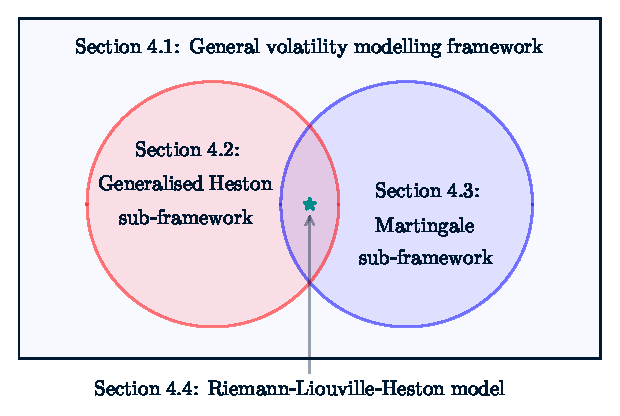
\includegraphics[width=0.60\linewidth]{figures/venn}
    \caption{Venn diagram showing the frameworks and model defined in \autoref{chap:framework}.}
    \label{fig:venn}
\end{figure}
\vspace{-4mm}

More specifically, \autoref{sec:heston_frame} defines a generalised Heston sub-framework in \autoref{def:gen_heston_frame}. In this sub-framework, models for a price $S$ and its cumulative variance $X$ verify equations
\begin{equation}\label{eq:gen_heston_intro}
    X'_t = \sigma Z_{X_t} + \kappa\left(\vt(t) - X_t\right) + v,\quad S_t = \exp\left(W^\rho_{X_t} - \tfrac12 X_t\right),
\end{equation}
where $\sigma,\kappa,v>0$, $\rho\in[-1,1]$ can be interpreted like the usual Heston parameters, $\vt$ is any bijective path in $\uC_0(\RR_+,\RR_+)$ and $Z=\{Z_x\}_{x\in\RR_+}$ a process with paths in $\uC_0(\RR_+,\RR)$. It is clear that this coincides with the classical Heston case in \autoref{eq:tce2} when $\vt(t)=\theta t$ and $Z=W^1$, but, unlike the Heston It\^o SDEs in \autoref{eq:heston_intro}, these models are well-defined over $\RR_+$ for \emph{any} $Z$ a.s.~verifying $\sup_{x\in\RR_+}\kappa x - \sigma Z_x = \infty$. This a.s.~condition simultaneously ensures the implicit random field in \autoref{eq:gen_heston_intro} is a.s.~in $\uG$ and that the c\`adl\`ag process $\bX$ which dominates $X$, analogous to that in \autoref{eq:ig_intro}, exists over the entirety of $\RR_+$.

The power of having this dominating process $\bX$, which derives \emph{directly} from a random field $Y$, is exhibited at the end of this section in \autoref{thm:mgf_existence} and \autoref{cor:gauss_heston_mgf}. These results provide conditions on $Z$ ensuring existence of the moment generating function (MGF) $M_X(p,t):=\EE[e^{pX_t}]$, which is important towards establishing the martingality of $S$ in \autoref{sec:martingale}. The second result focuses on Gaussian processes with sub-linear variance growth, like fractional Brownian motion, which due to \cite{gatheral_2018} and \cite{bayer_2016} are gaining prominence in volatility modelling and which we will make use of in \autoref{sec:RLH_model}.

In \autoref{sec:martingale} the focus is a sub-framework in which all price processes $S$ are martingales. Drawing primarily upon \cite{cont_2003} and \cite{guyon_2013}, the importance of martingales for derivative pricing is covered, with a strong emphasis on practicalities. Until this point, no restrictions have been placed on the relationship between a random field $Y$ and the Brownian motion $(W^0,W^1)$, except that both are random elements on $(\Omega,\cF,\PP)$, and so no restrictions on $X$ and $W^\rho$ defining $S$ through $S_t = \exp\left(W^\rho_{X_t} - \tfrac12 X_t\right)$. Culminating with \autoref{thm:price_martingale}, we now show how $Y$ should be adapted to the natural filtration $\{\cF_x\}_{x\in\RR_+}$ generated by $(W^0,W^1)$, to ensure that a price $S$ from the framework of \autoref{def:martingale_frame} is a $\cG_t:=\cF_{X_t}$-martingale on the filtered space $(\Omega,\cF,\{\cG_t\}_{t\in\RR_+},\PP)$.

Consistent with the models introduced thus far, the reality of stochastic interest rates are neglected in this martingale framework. Theoretically, this amounts to the assumption that interest rates are zero, so the usual bank account numeraire $B=\{B_t\}_{t\in\RR_+}$ is constant $B_t=B_0:=1$ and price processes $S$ coincide with their discounted counterpart $B^{-1}S$. See \cite{brigo_2006} and \cite{andersen_2010} for backgrounds to numeraires and discounting. In the future, a stochastic interest rate which is \emph{independent} from $W^\rho$ and $X$ may be introduced easily. Otherwise, it would be harmonious to link the interest rate's volatility to the price process's, e.g.~adopting a rate $r_X=\{r_{X_t}\}_{t\in\RR_+}$ adapted to $\{\cG_t\}_{t\in\RR_+}$ and bank account numeraire $B_t:=\exp(\int_0^t r_{X_s}\dd s)$, thus price process $S_t = B_t\exp(W^\rho_{X_t} - \tfrac12 X_t)$.

Returning to some of our motivations summarised by \autoref{eq:tce} and related to Doeblin's work, we clarify in passing that in this martingale sub-framework the random IVP solution $X$ defines a conventional time-change of the Brownian motion $W^\rho$, in the sense of \autoref{def:time_change}, consistent with \cite{revuz_1999}. A consequence of this is that our general definition $\sqrt{X'}$ of volatility coincides with the most conventional one in It\^o's calculus, depending on quadratic variations $[\cdot]$. Specifically, we can confirm that $[\log S]=X$ a.s.~holds.

At this point all of the probability theory is in place for practitioners to start defining models within our framework, which from the earlier pathwise analysis we know to be both very general and stable when compared with others. In \autoref{sec:RLH_model} the `Riemann-Liouville-Heston' (RLH) model is defined, which showcases both of the generalised Heston and martingale sub-frameworks because it resides in the intersection of these, as per \autoref{fig:venn}.

The idea behind this model is very simple, and is summarised by adapting \autoref{eq:tce} to
\begin{equation}
    X'_t = \sigma W^\alpha_{X_t} + \kappa\left(\theta t - X_t\right) + v,\quad S_t = \exp\left(W^\rho_{X_t} - \tfrac12 X_t\right),
\end{equation}
where we have simply replaced the Brownian motion $W^1$ with its Riemann-Liouville fractional derivative $W^\alpha:=D^\alpha(W^1)$ of some order $\alpha\in(0,\frac12)$, so the classical Heston model is recovered in the boundary case of $\alpha=0$. The fact that this replacement of Brownian motion is possible in our framework, without the need for any additional well-posedness analysis, should not be taken for granted, and is reminiscent of some of the motivations behind rough path theory given in the introductions of \cite{friz_2010} and \cite{friz_2014}. Given that, like $W^\alpha$, the variance process $X'$ becomes H\"older regular of orders in $(0,\frac12-\alpha)$, it is clear how to select the fractional derivative $\alpha$ in the RLH model to reproduce the evidence that volatility can exhibit H\"older regularities much lower than Brownian motion.

This model is specified fully in \autoref{def:RLH_model}, but before this a background to Riemann-Liouville fractional derivatives is provided, drawing upon theory from \cite{hardy_1928} to \cite{hamadouche_2000}. This theory proves important for establishing the convergence of a simulation scheme for the purpose of derivative pricing, which is the general focus of \autoref{sec:vol_surfaces}. This scheme is used to generate the implied volatilities at the end of \autoref{sec:vol_surfaces}, which are contrasted with those of the classical Heston model, demonstrating desirable features such as power-law scaling of skews (discussed in the \hyperlink{prologue}{Prologue}) and curvatures, as exhibited by leading rough volatility models. Standalone and simplified \texttt{python} code for this simulation scheme is provided in the \hyperlink{appendix}{Appendix}, with seeded output shown in \autoref{fig:simulation_output}.

The final goal is to use the RLH model to illustrate the pathwise limiting results of \autoref{chap:solutions}, and to specialise these to the classical Heston model in order to precisely answer our motivating questions in the \hyperlink{prologue}{Prologue}. The most striking findings in \autoref{sec:price_limits} are as follows.

First let $S^n$ be the classical Heston process in \autoref{thm:mech_pro}, define $X^0$ to be the IG process in both \autoref{eq:nig_prologue} and \autoref{eq:ex_nig_pro}, and define the c\`adl\`ag and interval-valued processes
\begin{multline}\label{eq:intro_limit_def}
    S^\circ_t := \exp\left(\sqrt{1-\rho^2}W^0_{X^0_t} + \frac{2\rho-\sigma}{2\sigma}X^0_t -\frac{\rho\theta}{\sigma} t\right), \\
    S^\bullet_t := \bigg\{\exp\left(W^\rho_x - \frac12 x\right) : x\in[X^0_{t_-},X^0_t] \bigg\}.
\end{multline}
Then $S^\circ$ is the exp-NIG process in \autoref{thm:mech_pro}, while $S^\bullet$ is a stochastic counterpart of the interval-valued path $w\bullet\bvp$ from \autoref{eq:excursion_path}. The inclusion $S^\circ_t\in S^\bullet_t =:[S^-_t,S^+_t]$ becomes clear following \autoref{lem:NIG_reduc}, which clarifies the counter-intuitive representation $S^\circ_t=\exp(W^\rho_{X^0_t} - \frac12 X^0_t)$, and from which $S^\bullet_t=\{S^\circ_t\}$ almost everywhere (a.e.) follows, meaning $S^-_t=S^\circ_t=S^+_t$. Then, although we show that the convergence in \autoref{thm:mech_pro} can be extended to \emph{either} the convergence of finite-dimensional distributions of $S^n$ to $S^\circ$ \emph{or} the pointwise convergence a.e.~in time on a.e.~path, the graphs of $S^n$ in $\RR_+\times\RR$ actually converge weakly to that of $S^\bullet$ with respect to the Hausdorff distance in \autoref{cor:heston_hausdorff}. So $S^n$ develops compact spatial excursions, of size $S^+_t - S^\circ_t$ upwards and  $S^\circ_t - S^-_t$ downwards, which are almost nowhere but nevertheless dense in time, like the discontinuities of $X^0$. \autoref{fig:hausdorff_composite} helps tremendously to visualise (and validate) this peculiar kind of Hausdorff convergence.

\vspace{3mm}\textbf{\autoref{chap:conclusion}: Conclusion.} Although we did not set out to explore the volatility modelling frameworks of \autoref{chap:framework}, with these instead revealing themselves over several years when considering the questions finally answered in \autoref{sec:price_limits}, we have by this point made a convincing case for the value of our spatially irregular IVPs from \autoref{prob:ivp2} in finance. But actually it is clear that these can theoretically benefit the modelling of any dynamical system, given that the bijective solutions, which we label cumulative variance paths in our context, essentially model time itself, which is by definition central to all dynamical systems.

Unlike in other fields, the modelling of time itself is a very natural concept in finance, which many authors have exploited, mostly with subordinated L\'evy processes, like \cite{barndorff-nielsen_2001a}, \cite{geman_2001}, and \cite{carr_2004} to name a few. This is because the prices which we aim to model are \emph{fundamentally} observed parametrically, with both the temporal and spatial components of a trade, both appearing random, being indexed by another notion of time captured by deterministic trade identifiers.

For applications in other fields, the general time-irreversibility of our IVPs, clarified in \autoref{chap:solutions}, is peculiarly consistent with apparent asymmetries in nature between future and past, which is related to the strict increase of entropy and second law of thermodynamics. Of course we leave such exciting general considerations for the future, and in \autoref{chap:conclusion} focus on several more specific ideas for future financial research which this thesis has made possible. This ranges from theoretical `Carath\'eodory' extensions of the ODEs treated here, to the practical implications of the surprising interval-valued limits like $S^\bullet$ in \autoref{eq:intro_limit_def}.

\vspace{3mm}\textbf{\hyperlink{epilogue}{Epilogue}: Integrated CIR-L\'evy relationships.} As discussed briefly already, the \hyperlink{epilogue}{Epilogue} consolidates and generalises what we consider to be the origin of the Heston and NIG limiting relationship, entirely from the perspective of It\^o SDEs. This is presented purely from this more accessible perspective, although our proofs of course require random IVPs.

To this end, we first drastically over-parameterise Heston's CIR SDE, in accordance with
\begin{equation}
    \dd V^n_t = n^\alpha a \sqrt{V^n_t}\dd W_t + n(b - n^{\beta-1} V^n_t)\dd t,\quad V^n_0=n^\gamma c.
\end{equation}
The exponents $\alpha,\beta,\gamma\in(-\infty,1]$ then control how each term scales as $n\to\infty$ in comparison with the reversionary term $nb$, and specific selections are provided which coincide with the regimes of \cite{heston_1993}, \cite{fouque_2011} and \cite{mechkov_2015}. Depending on the selection of these exponents, \autoref{tab:cir_limits} identifies the eight possible L\'evy processes which arise from the integrated CIR process. Two of these are degenerate, but also two arise with random starting points. So not only does this thesis accommodate continuous, rough and jump models of volatility through the novel application of random IVPs, but here we find randomised models arising as well, as studied in \cite{mechkov_2016} and \cite{jacquier_2019}.
